\newpage
\subsection{Отгрузка готовой продукции}
\label{bp:Shipment}

Кладовщик получает от логиста печатную версию плана отгрузок (рис. \ref{pic:X.2}). Но план отгрузок может быть нарушен менеджерами по продажам. Менеджер по продажам может потребовать загрузить транспорт вне очереди. 

В системе 1С: УПП производится учет простоя транспорта в ожидании погрузки/разгрузки, в котором так же фиксируется время погрузки/разгрузки.  Отчет ''Выполнение норм пребывания машин на территории ПЗБМ Филиал Веста'' представлен на рис. \ref{pic:IX.1.,.}.

Водители автотранспорта отмечают у охранника на проходной ПРЕДПРИЯТИЯ время прибытия и перед заездом на территорию получают проездной лист (создается в системе 1С: УПП) и инструкцию.
% (рис. \ref{pic:IX.2.}). 
Заезд автотранспорта осуществляется по плану погрузки.

Кладовщик совместно с водителем погрузчика находит необходимую к отгрузке готовую продукцию. Отгрузка производится по номенклатуре, а не по заказам. 

Продукция, которая была произведена ранее не будет отгружена, т.к. паллеты могут быть заставлены на складе. При этом менеджер по продажам может прислать по электронной почте требование переклеить бирки на паллетах при отгрузке, данные бирки не занесены в систему 1С: УПП и в технологические карты (рис. \ref{pic:IX.10}). В этом случае упаковка паллет вскрывается, при погрузке сканируются и изымаются первоначальные бирки и вставляются бирки, которые прислал менеджер по продажам. Кладовщики совместно с водителями погрузчиков производят повторную упаковку паллет прямо на складе (рис. \ref{pic:Х упаковка на складе}). 

При погрузке кладовщики сканируют с помощью терминала сбора данных штрих-коды  на каждой паллете. Водители погрузчиков производят расстановку паллет согласно схеме погрузки, которая создается менеджером по логистике. Кладовщик делает пометки о факте отгрузки в печатной версии плана погрузки (рис. \ref{pic:IX план погрузки}). Если упаковка и размеры паллеты не соответствуют технологической карте, то в системе 1С: УПП оформляется накладная на перемещение и паллет возвращается на производство (рис. \ref{pic:IX.13}).   Каждую операцию по погрузке/разгрузке автотранспорта фиксируют в печатном бланке ''Учет погрузочно-разгрузочных работ'' (рис. \ref{pic:IX.8}). Бланк никуда не перередается, а используется для сверки и контроля. После завершения отгрузки кладовщик формирует в системе 1С: УПП и печатает документы реализации (рис. \ref{pic:IX памятка кладовщикам}).
Ежедневно утром все документы по отгрузке и реализации за прошедшие сутки сдаются в бухгалтерию. Бухгалтер проверяет ''Расходный ордер'' созданный кладовщиком, производит выгрузку документов реализации из системы 1С: УПП в 1С: Бухгалтерия.  
Кладовщик печатает из системы 1С: УПП паспорт качества и сертификаты на готовую продукцию.
%\clearpage
%Инженер по отгрузке передает план отгрузки на склад кладовщику.  Инженер в СБИС формирует пропуск (распоряжение), указывает машину из системы СБИС .


%Водитель едет на склад с распоряжением, передает распоряжение кладовщику. Кладовщик проверяет остатки по готовой продукции в системе СБИС и в распоряжении, делает копию распоряжения. С копией распоряжения кладовщик выполняет погрузку готовой продукции в транспорт. Кладовщик находит паллеты с готовой продукцией на складе согласно распоряжения.

%На бирке с готовой продукцией нет полной информации по продукции.
%Кладовщик ищет только по наименованию заказчика и наименованию изделия. Нередко кладовщику приходится вскрывать упаковки для сверки наименования печати изделия. Кладовщик указывает водителю погрузчика какие паллеты грузить в транспорт.


%Кладовщики в системе СБИС создает на основании распоряжения на отгрузку документ ''Расходная накладная''. Строки документа будут скопированы автоматически. Кладовщик из системы СБИС печатает сопроводительные документы: ТН, ТТН, паспорт качества.

%\newpage

\begin{figure}
\begin{center}
 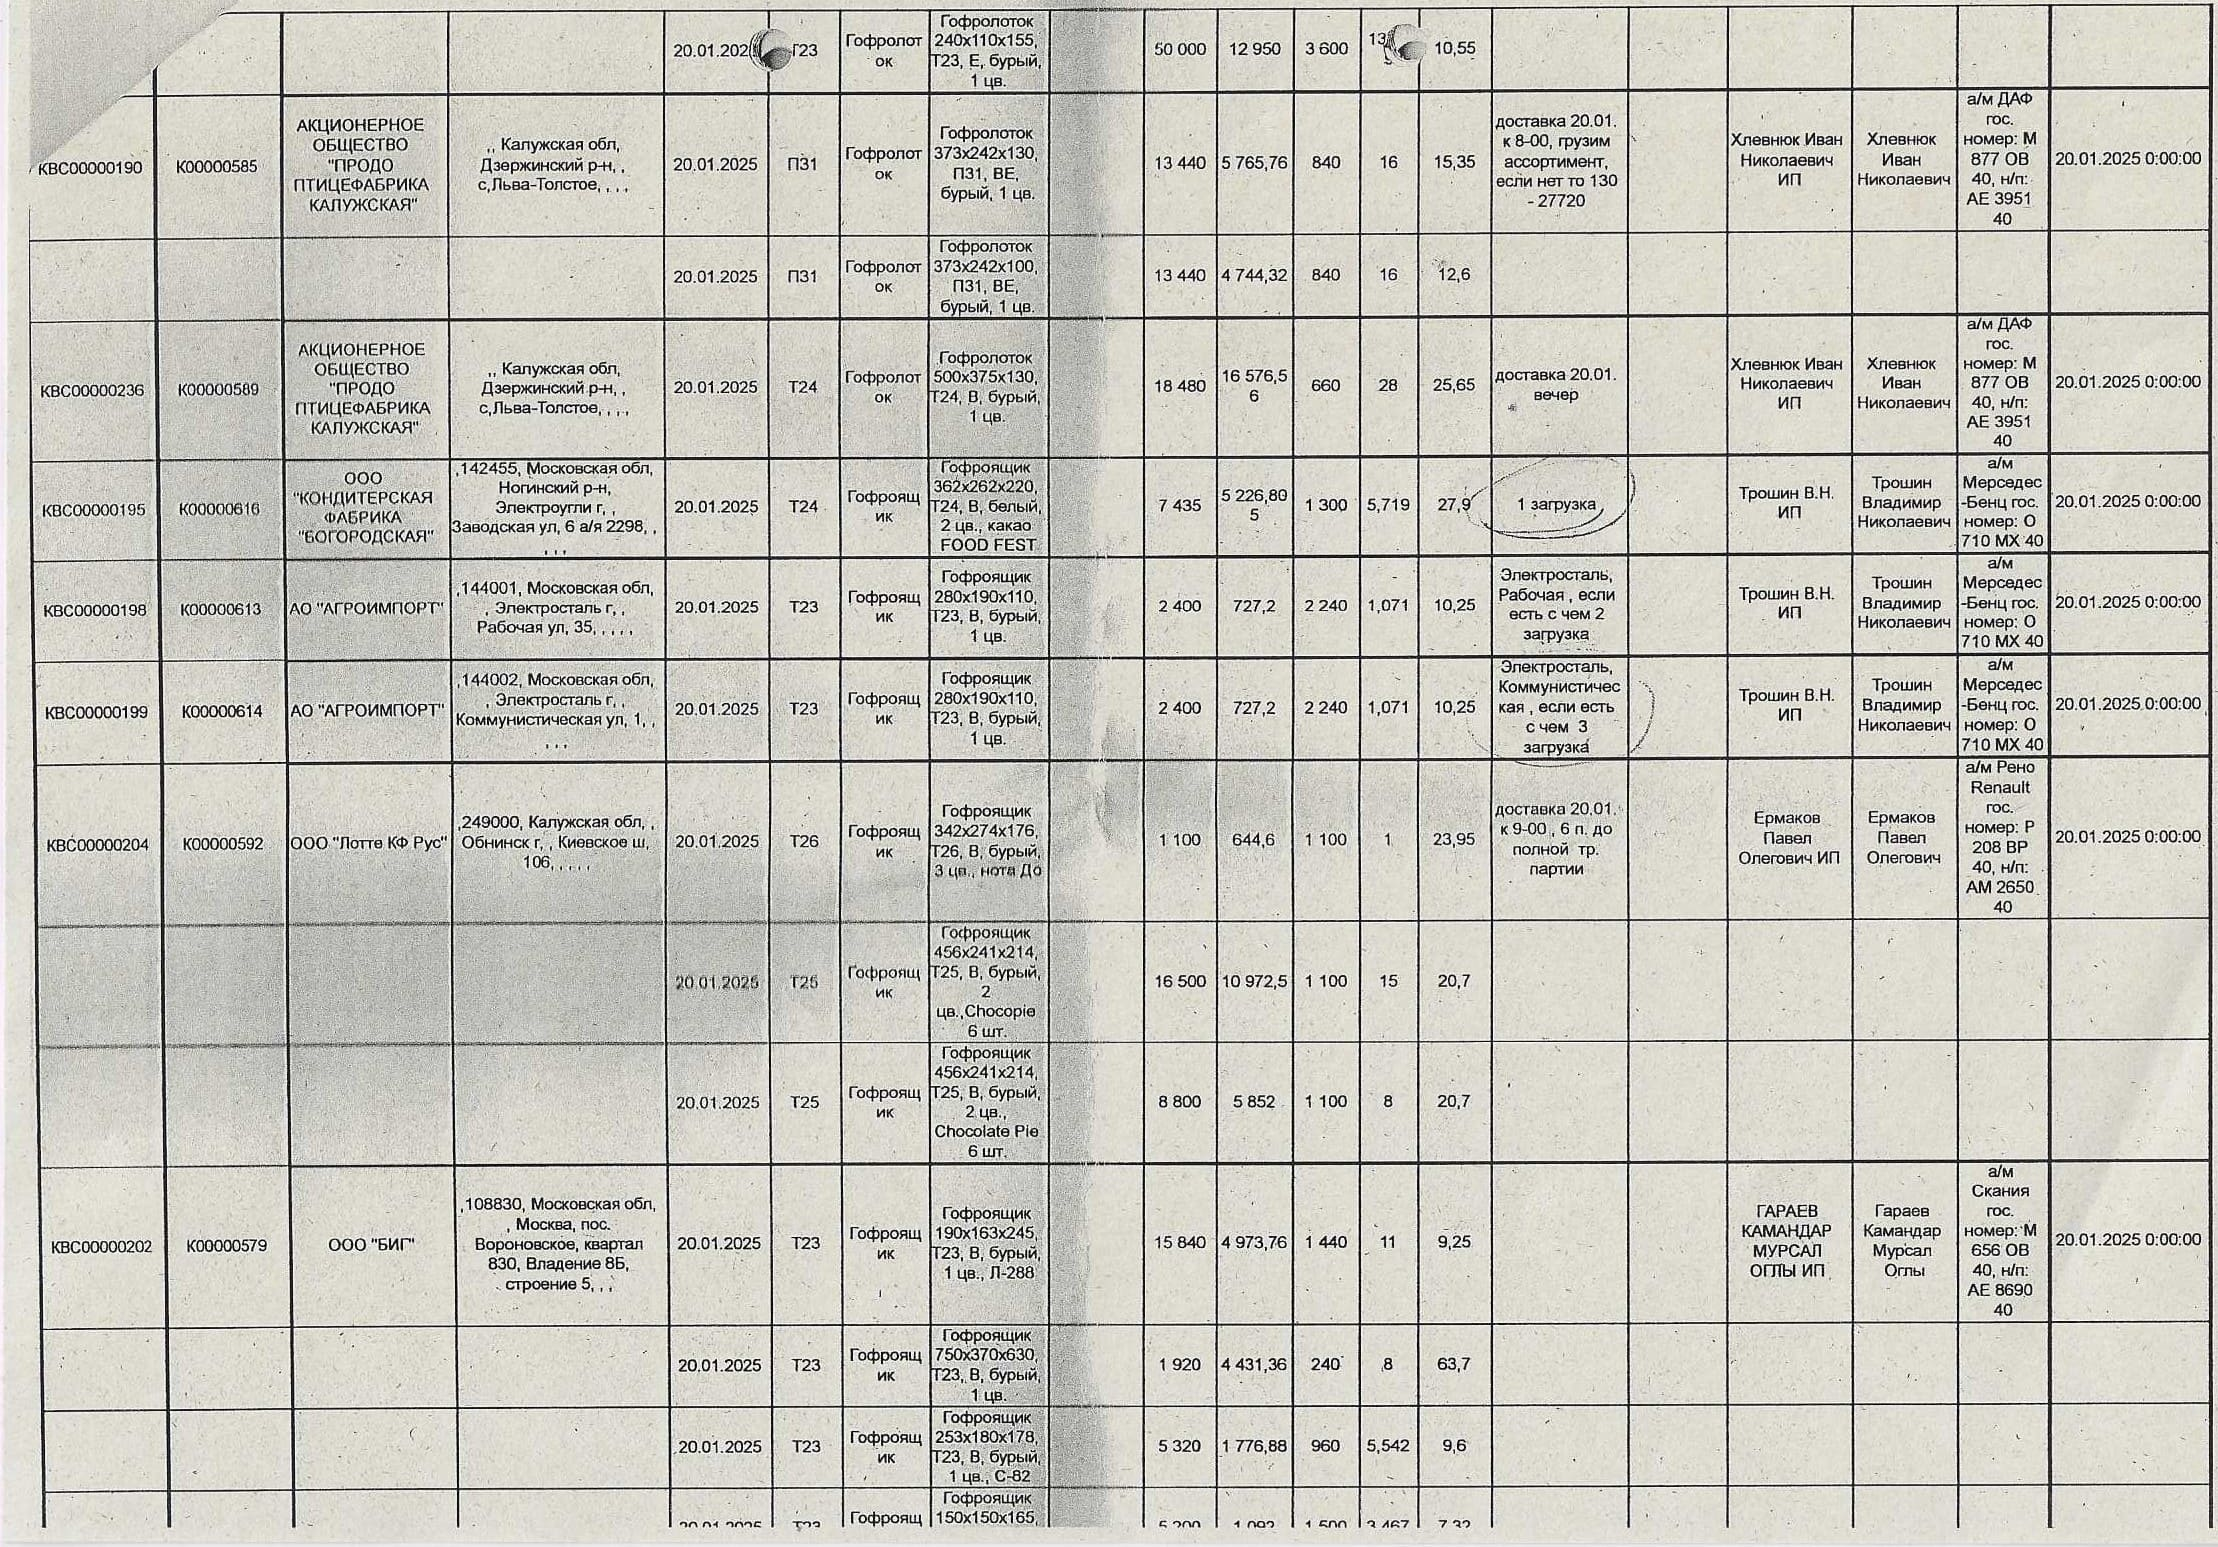
\includegraphics[height=0.5\textheight, angle=90, keepaspectratio]{Pics/X.2.jpg}
\end{center}
 \caption{План отгрузки}
 \label{pic:X.2}
\end{figure}

\begin{figure}
\begin{center}
 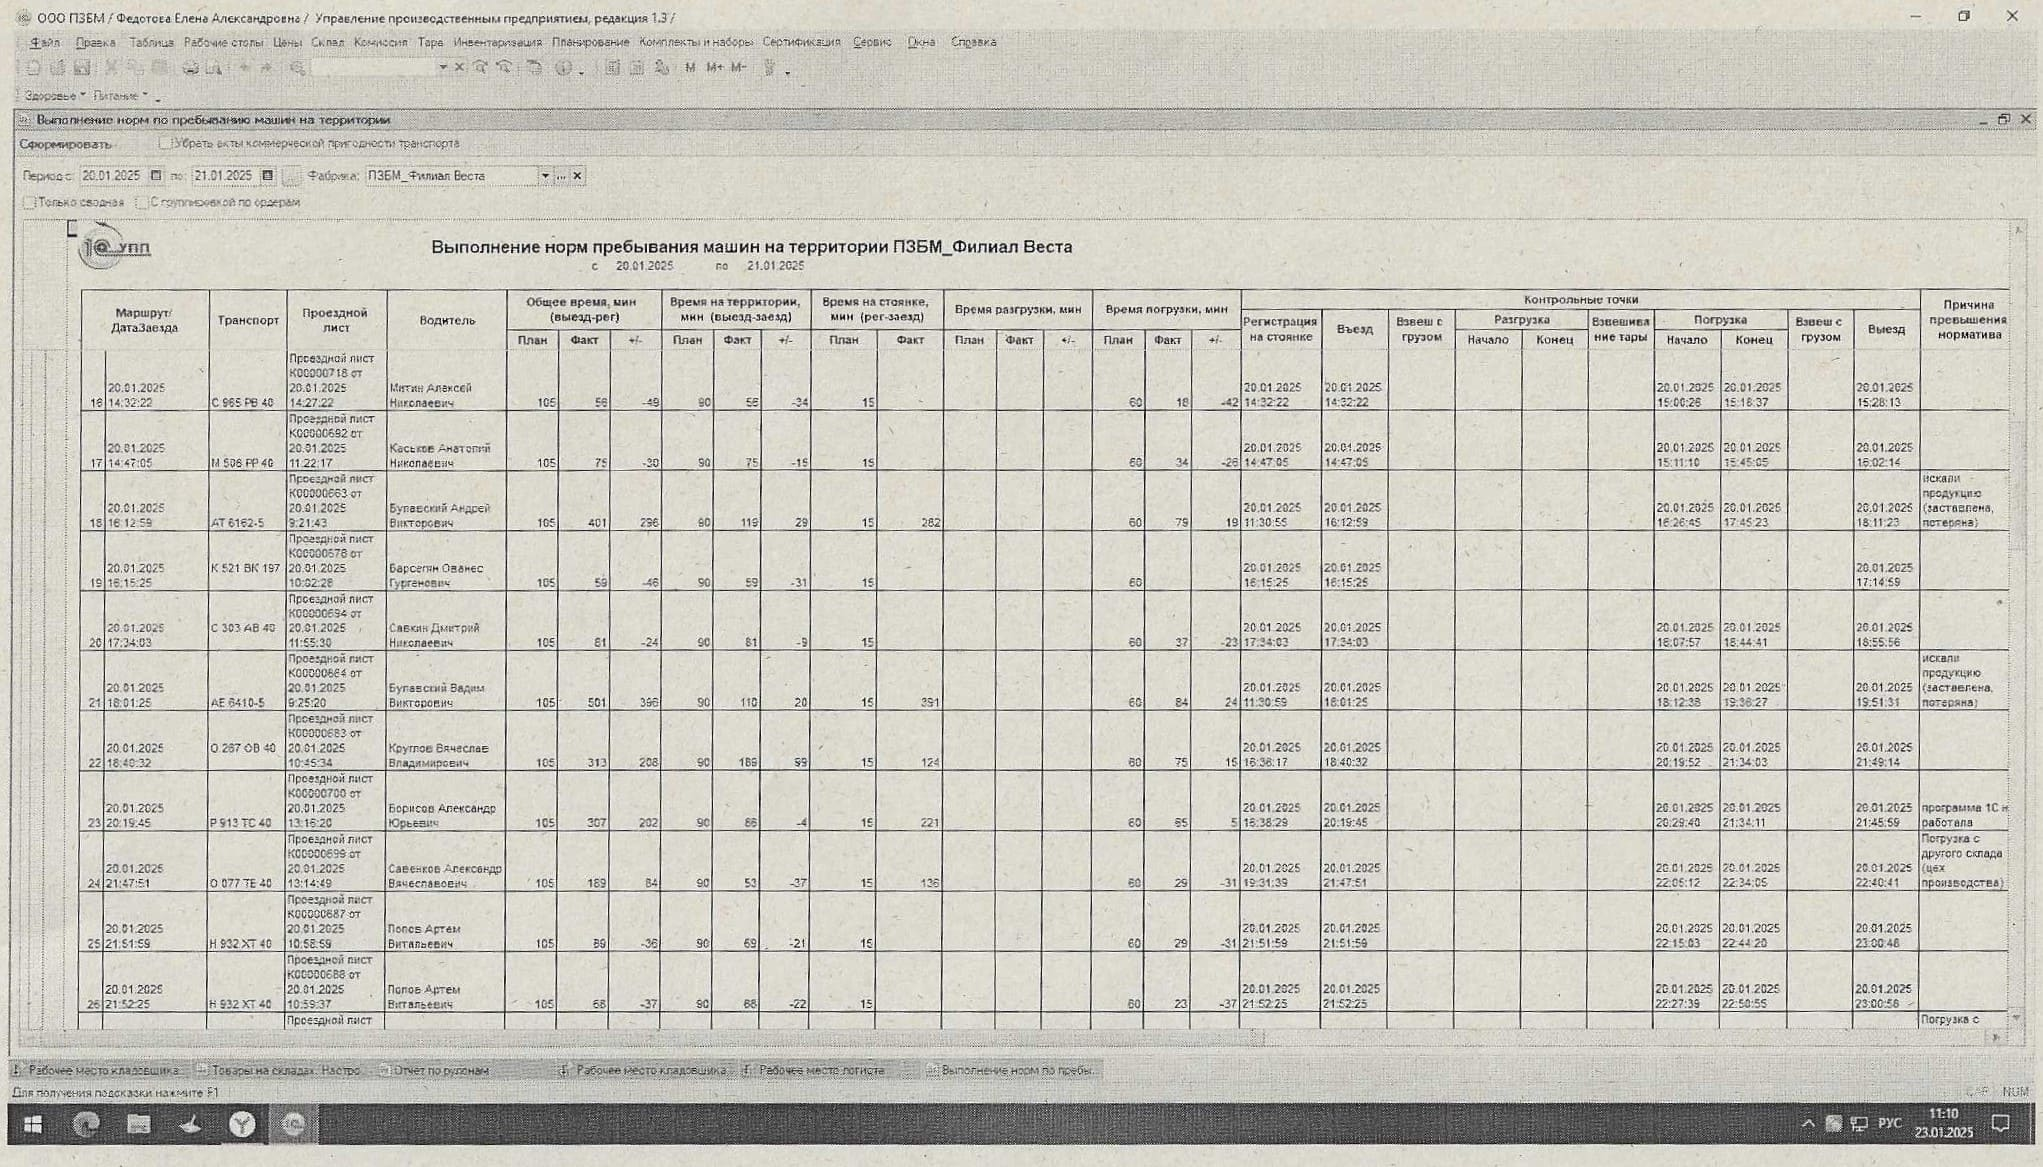
\includegraphics[height=0.5\textheight, angle=90, keepaspectratio]{Pics/IX.1.,..jpg}
\end{center}
 \caption{Выполнение норм пребывания машин}
 \label{pic:IX.1.,.}
\end{figure}

% \begin{figure}
% \begin{center}
%  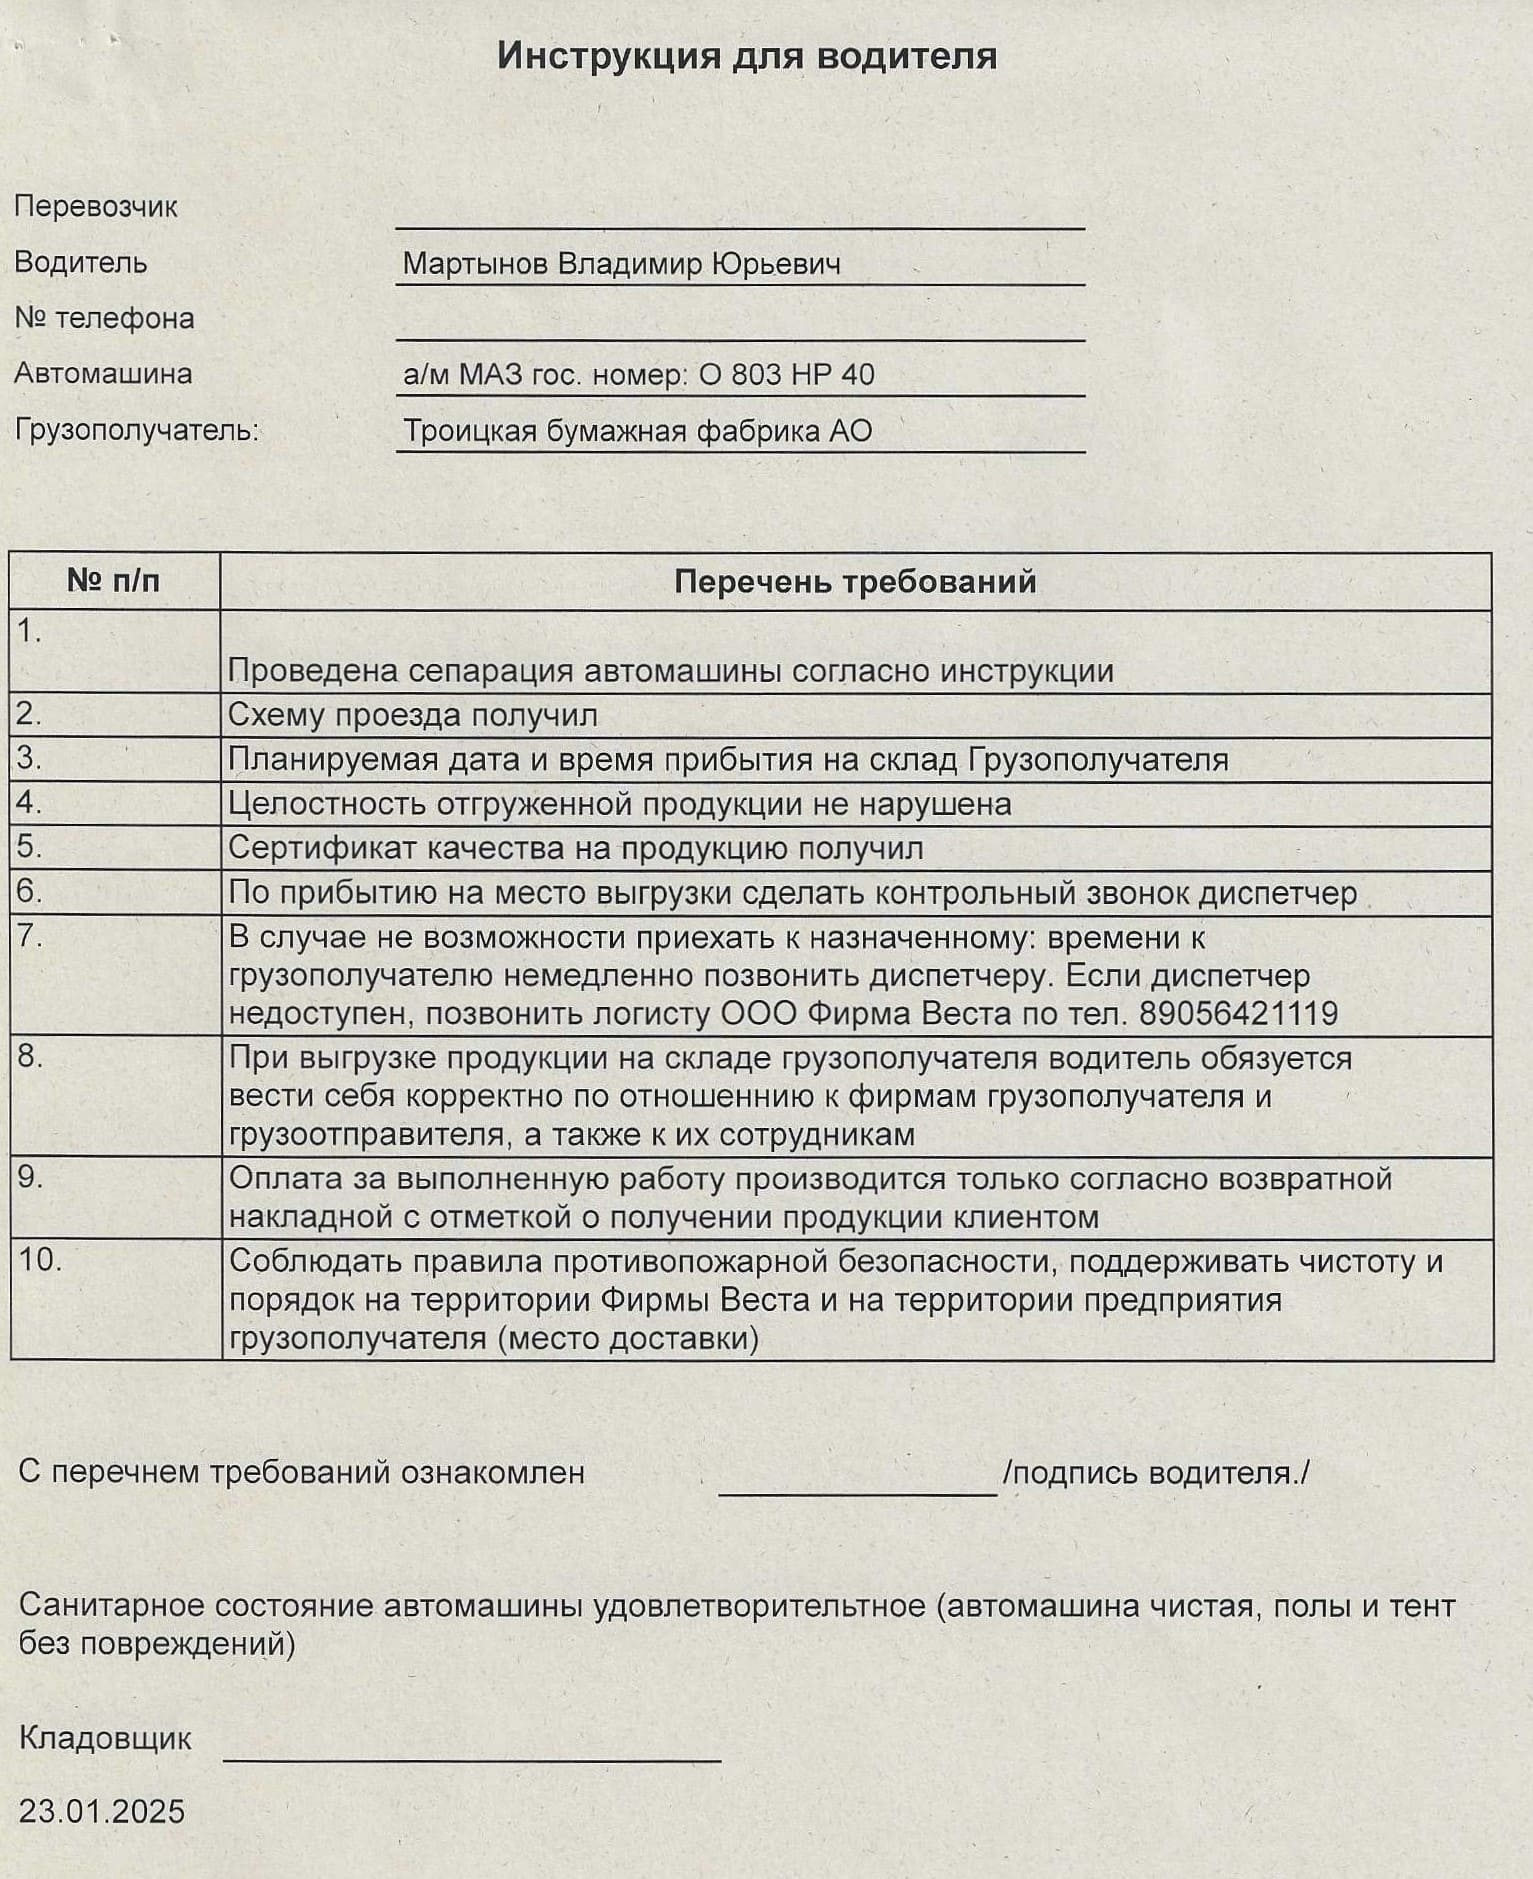
\includegraphics[height=0.8\textheight, keepaspectratio]{Pics/IX.2..jpg}
% \end{center}
%  \caption{Инструкция для водителя}
%  \label{pic:IX.2.}
% \end{figure}

\begin{figure}
\begin{center}
 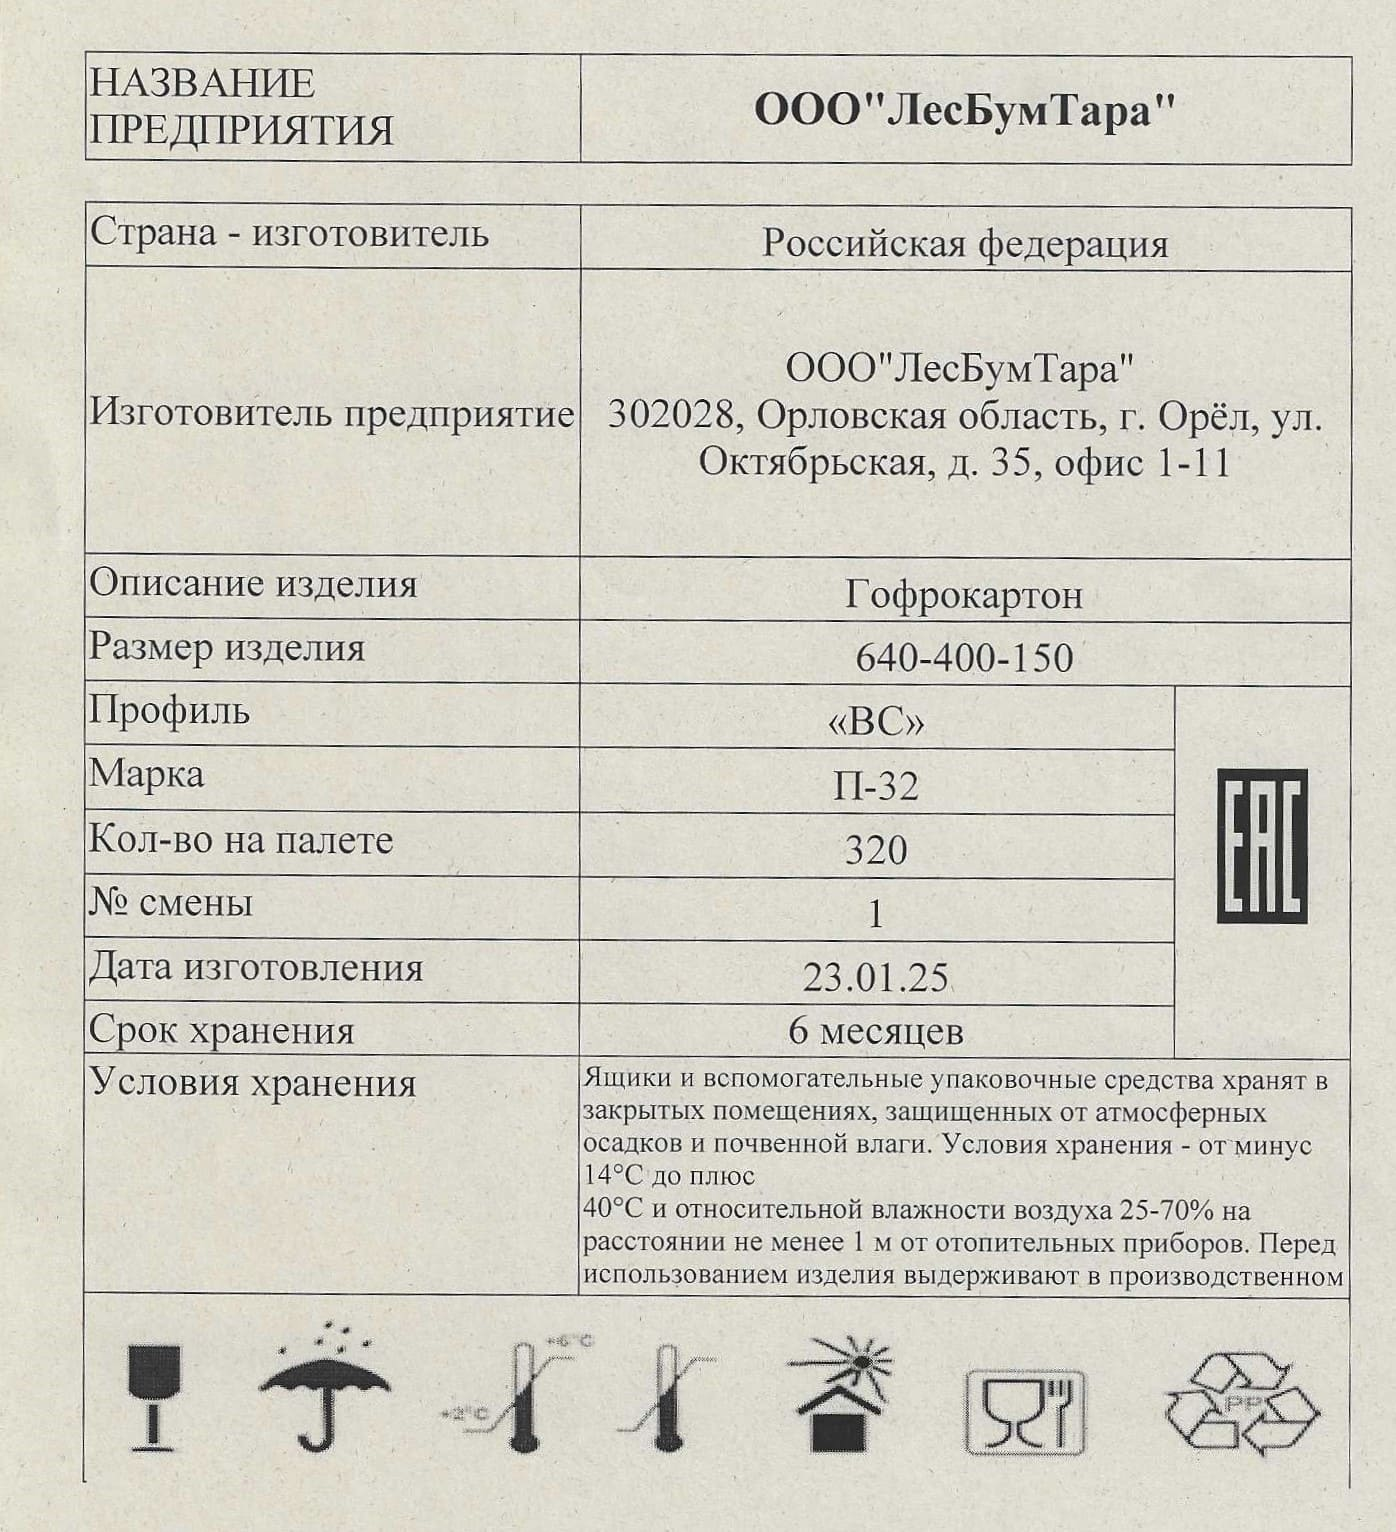
\includegraphics[height=0.7\textheight, keepaspectratio]{Pics/IX.10.jpg}
\end{center}
 \caption{Новая бирка}
 \label{pic:IX.10}
\end{figure}

\begin{figure}
\begin{center}
 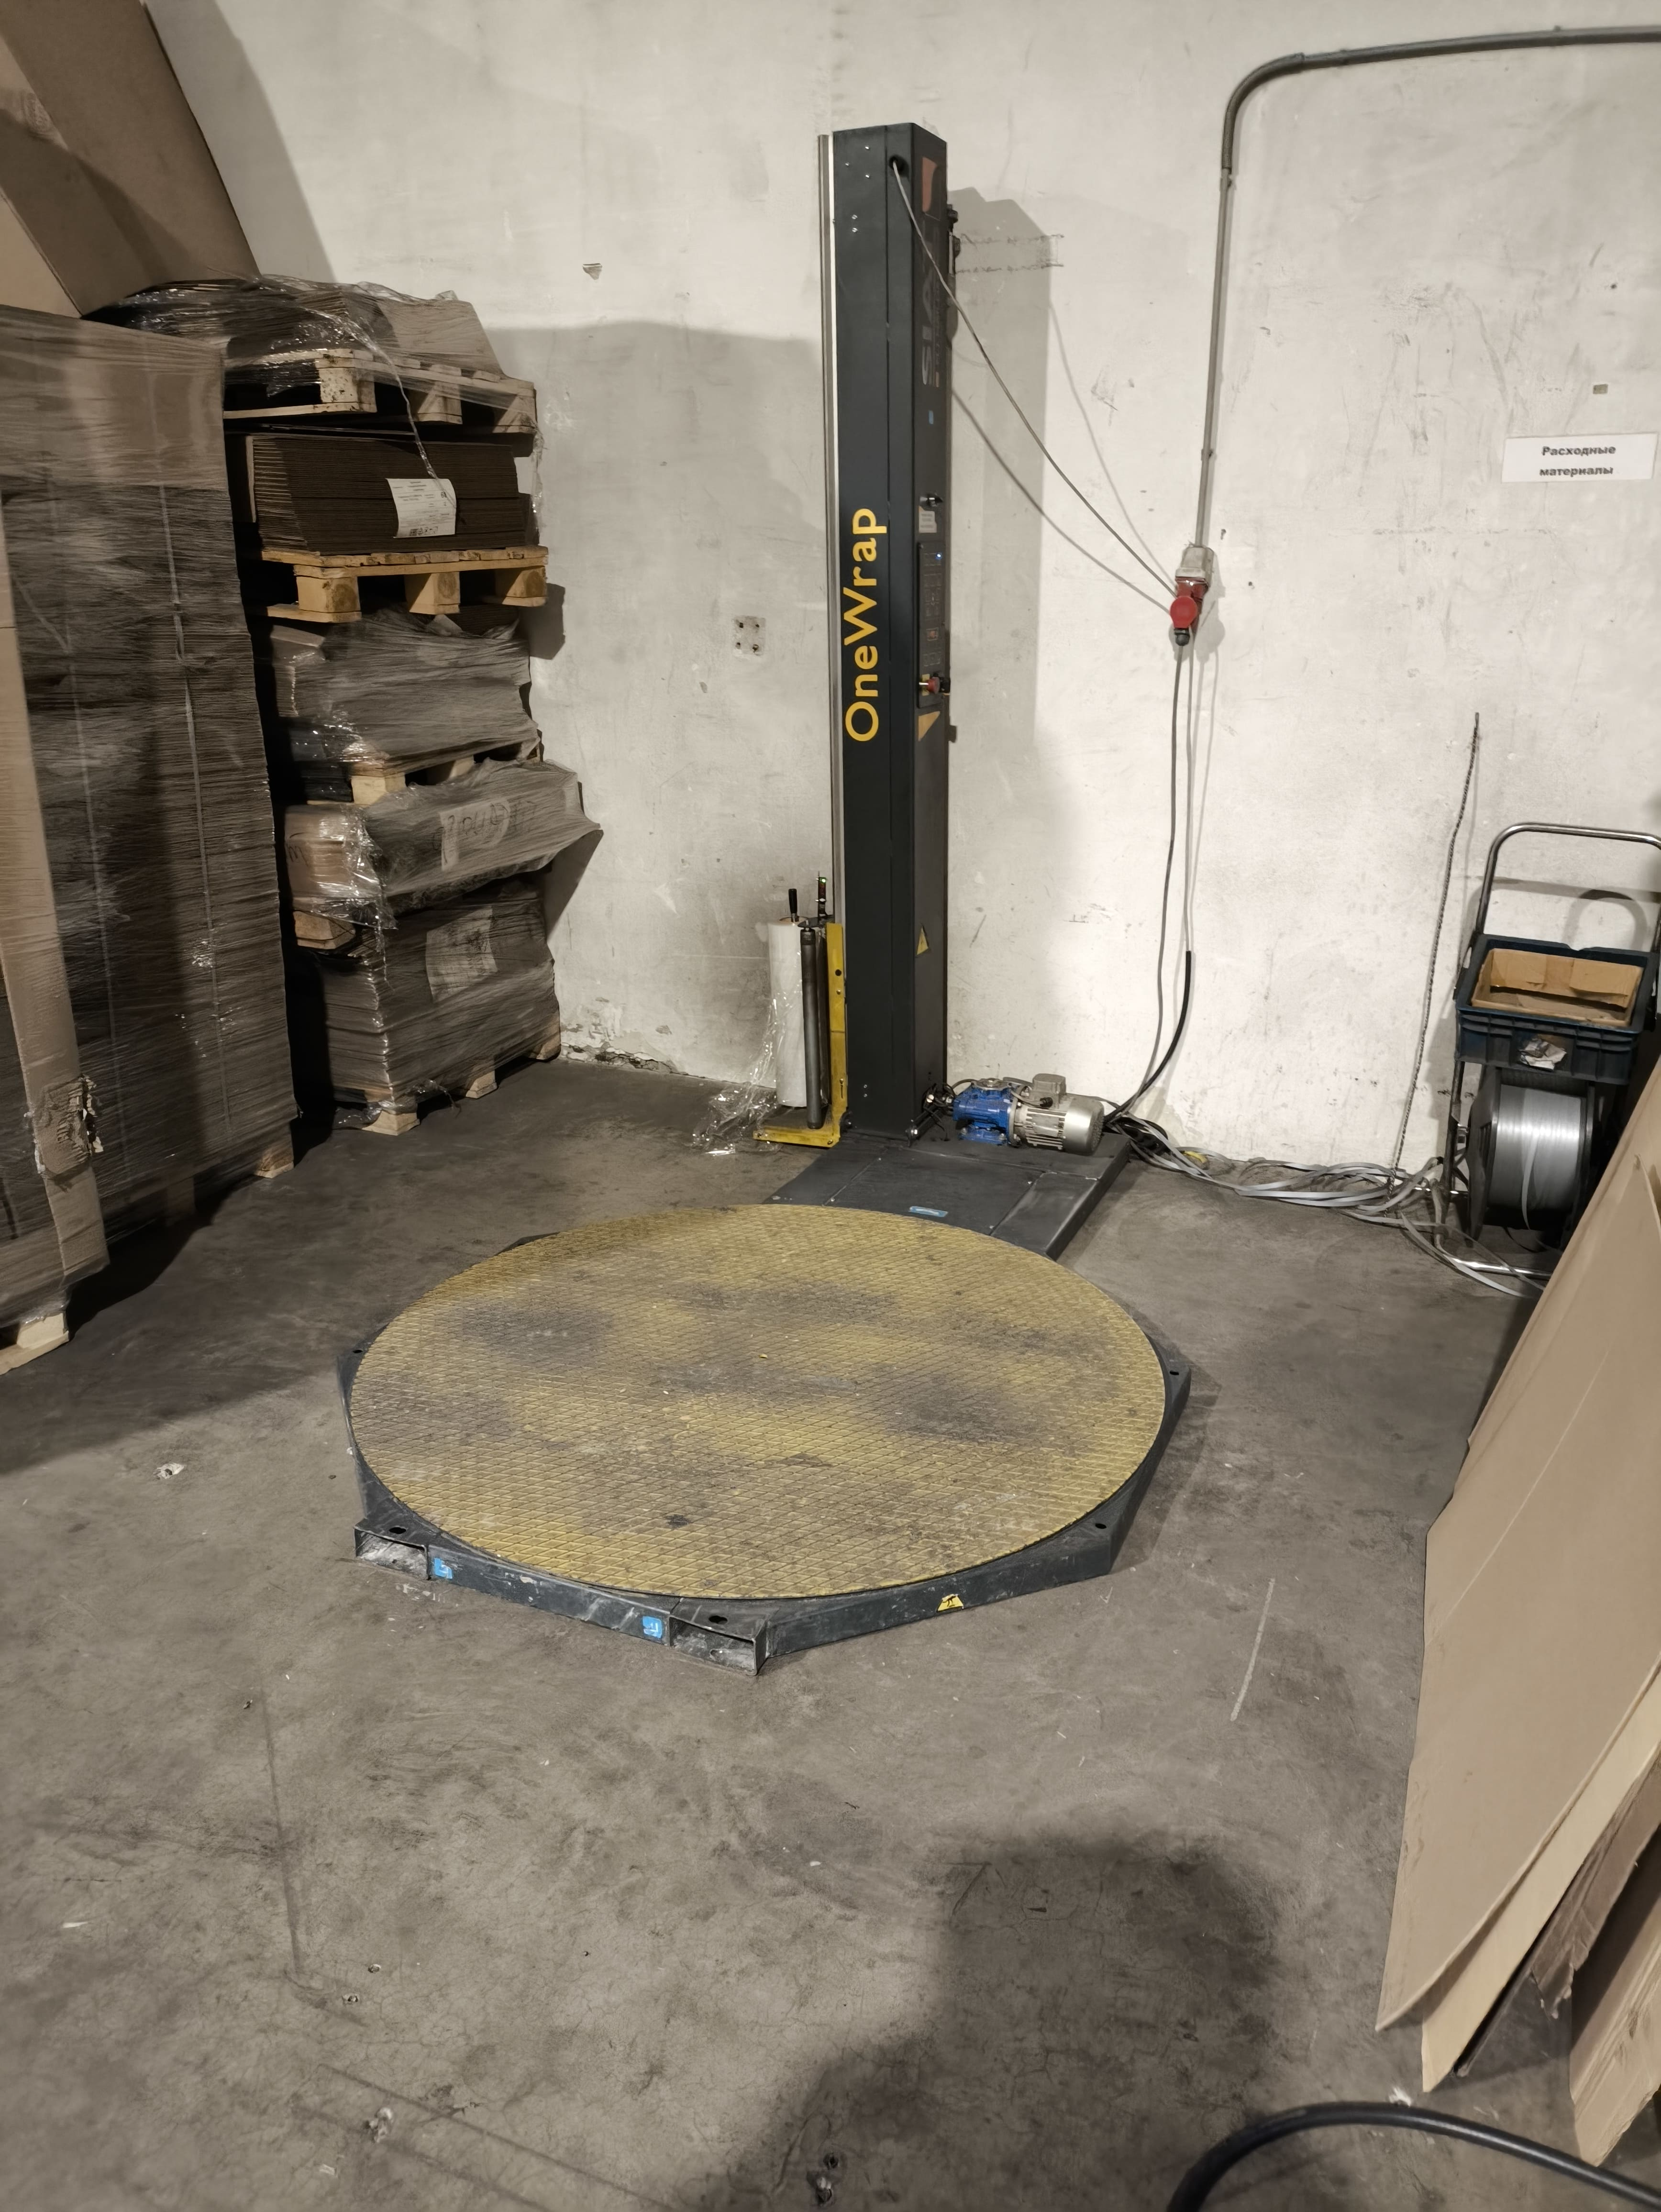
\includegraphics[height=0.7\textheight, keepaspectratio]{Pics/Х упаковка на складе.jpg }
\end{center}
 \caption{Паллетировщик на складе}
 \label{pic:Х упаковка на складе}
\end{figure}

%\begin{center}
% \includegraphics[height=0.4\textheight, keepaspectratio]{Pics/Х схемы погрузки.jpg }
%\end{center}
% \caption{Справочник схем погрузки в 1С: УПП}
% \label{pic:Х схемы погрузки}
%\end{figure}

\begin{figure}
\begin{center}
 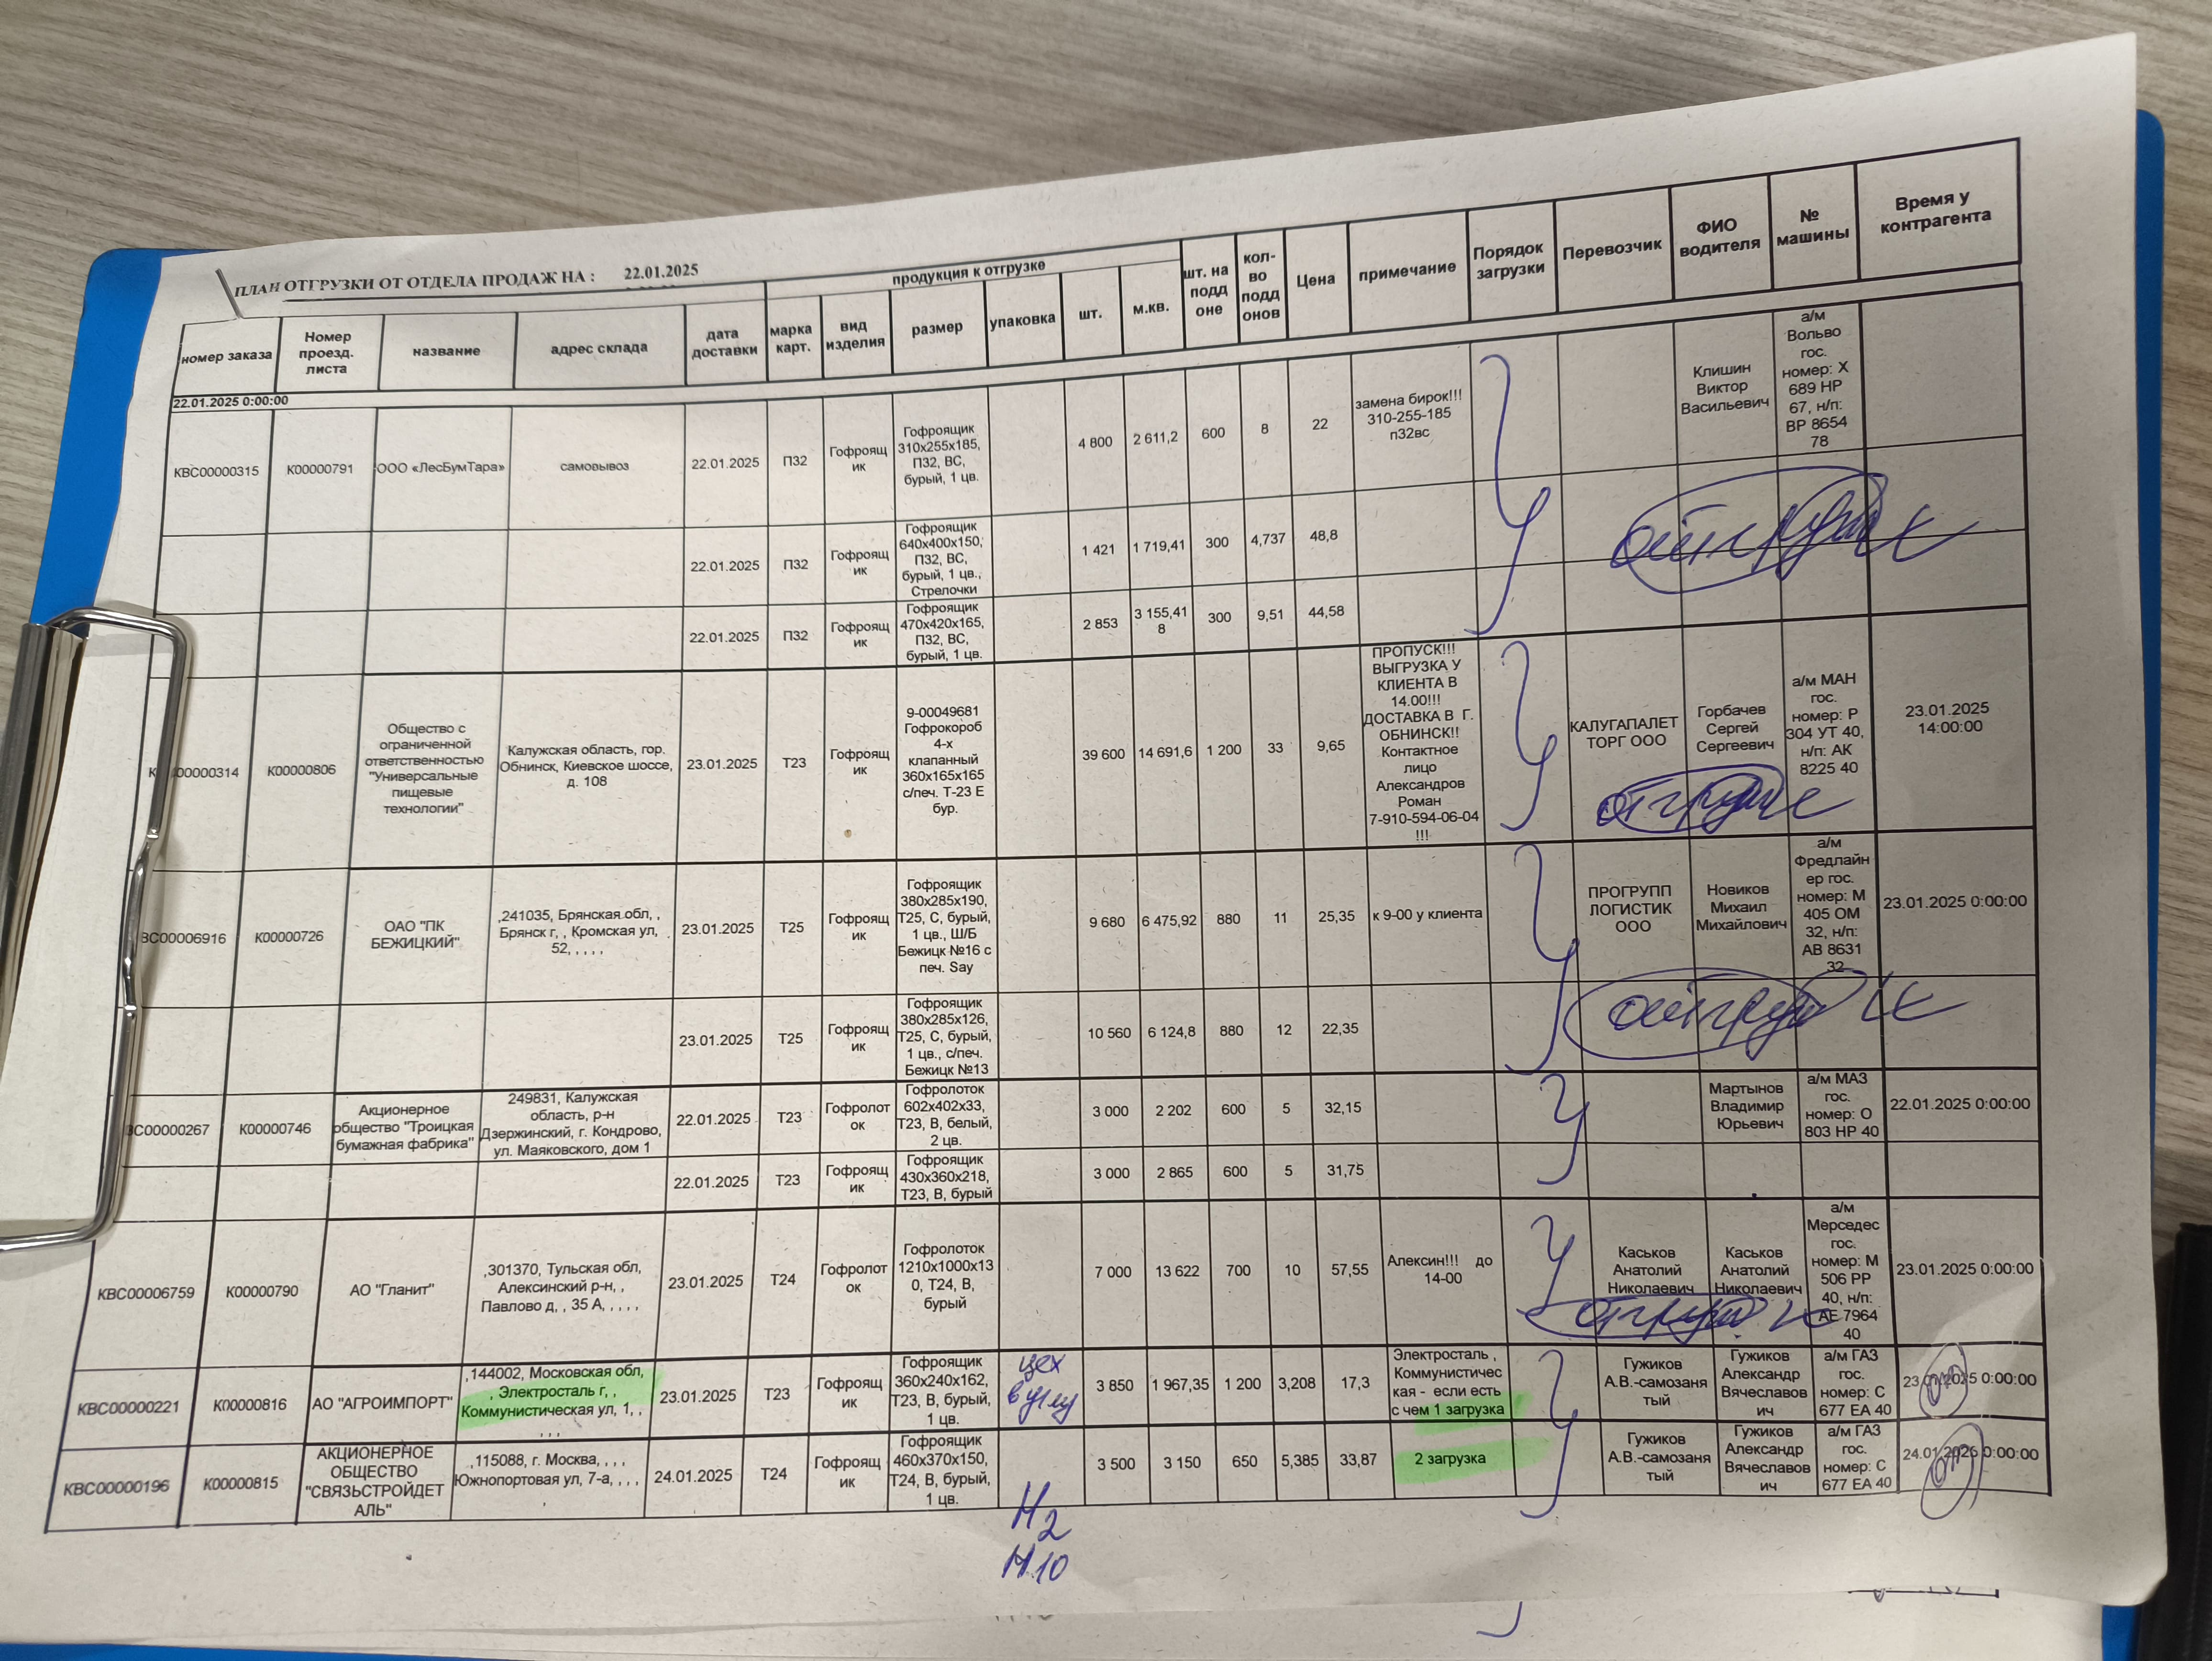
\includegraphics[height=0.4\textheight, keepaspectratio]{Pics/IX план погрузки.jpg }
\end{center}
 \caption{План погрузки с отметками кладовщика}
 \label{pic:IX план погрузки}
\end{figure}

\begin{figure}
\begin{center}
 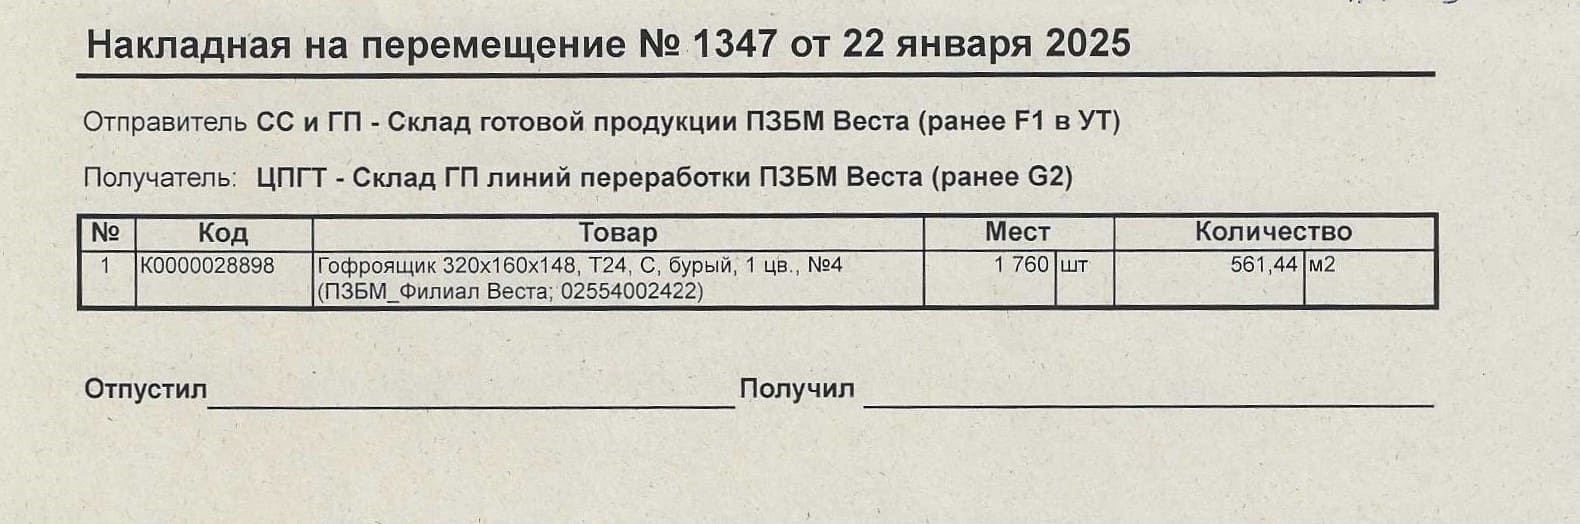
\includegraphics[height=0.22\textheight, keepaspectratio]{Pics/IX.13.jpg }
\end{center}
 \caption{Накладная на перемещение}
 \label{pic:IX.13}
\end{figure}

\begin{figure}
\begin{center}
 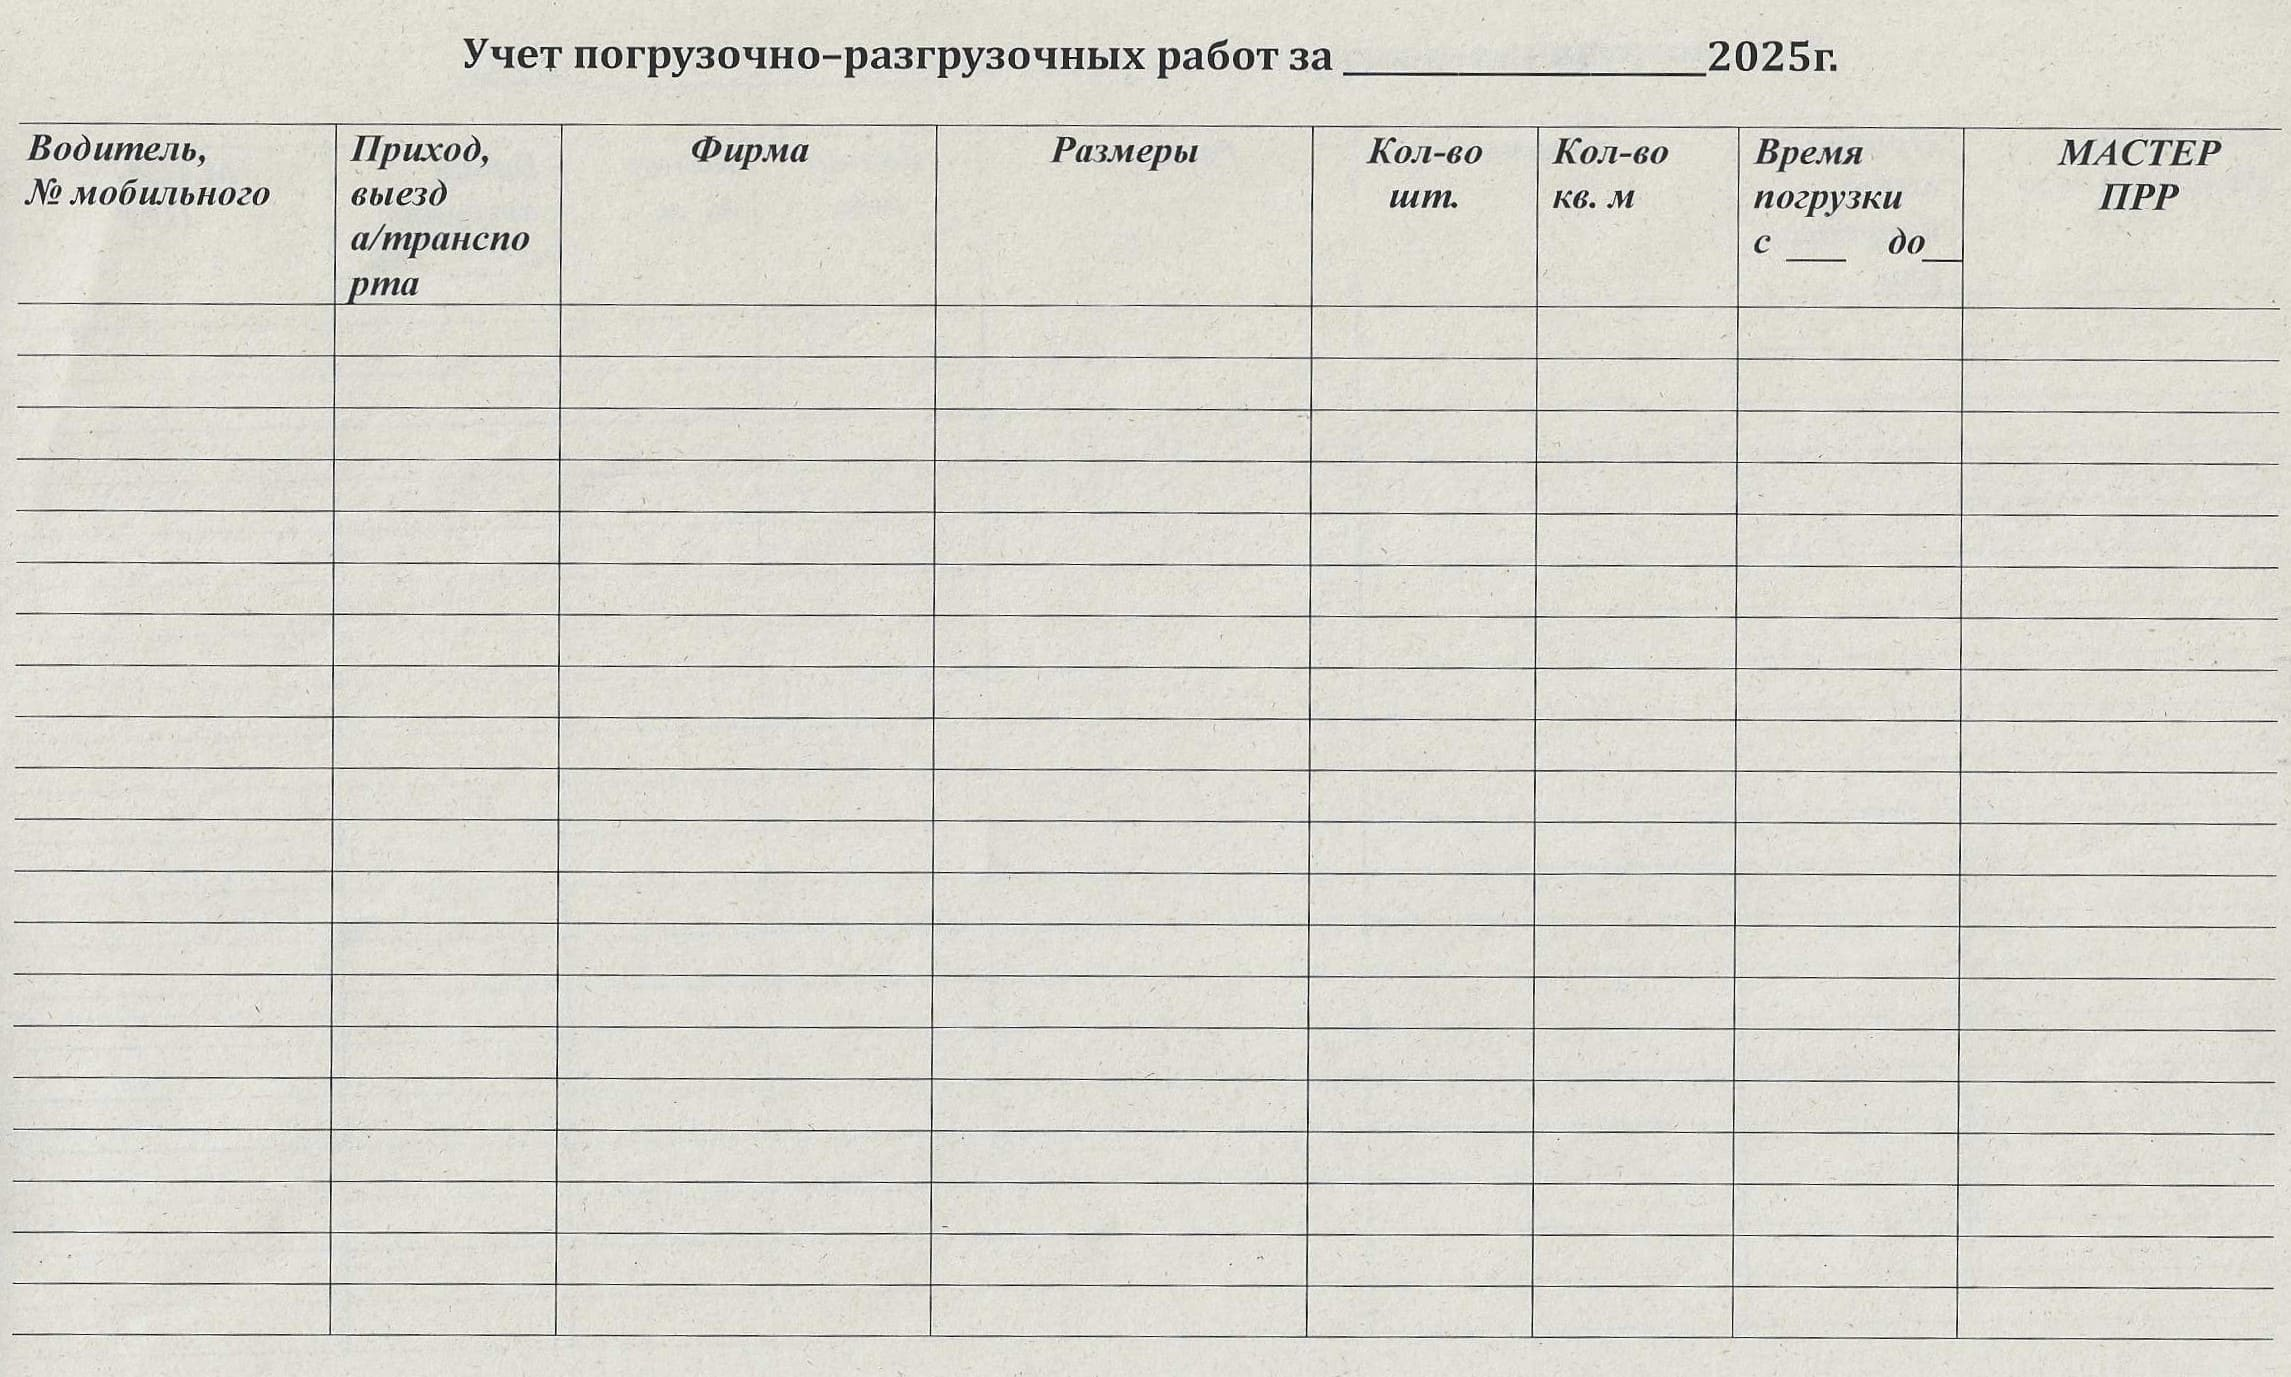
\includegraphics[height=0.4\textheight, keepaspectratio]{Pics/IX.8.jpg }
\end{center}
 \caption{Учет погрузочно-разгрузочных работ}
 \label{pic:IX.8}
\end{figure}

\begin{figure}
\begin{center}
 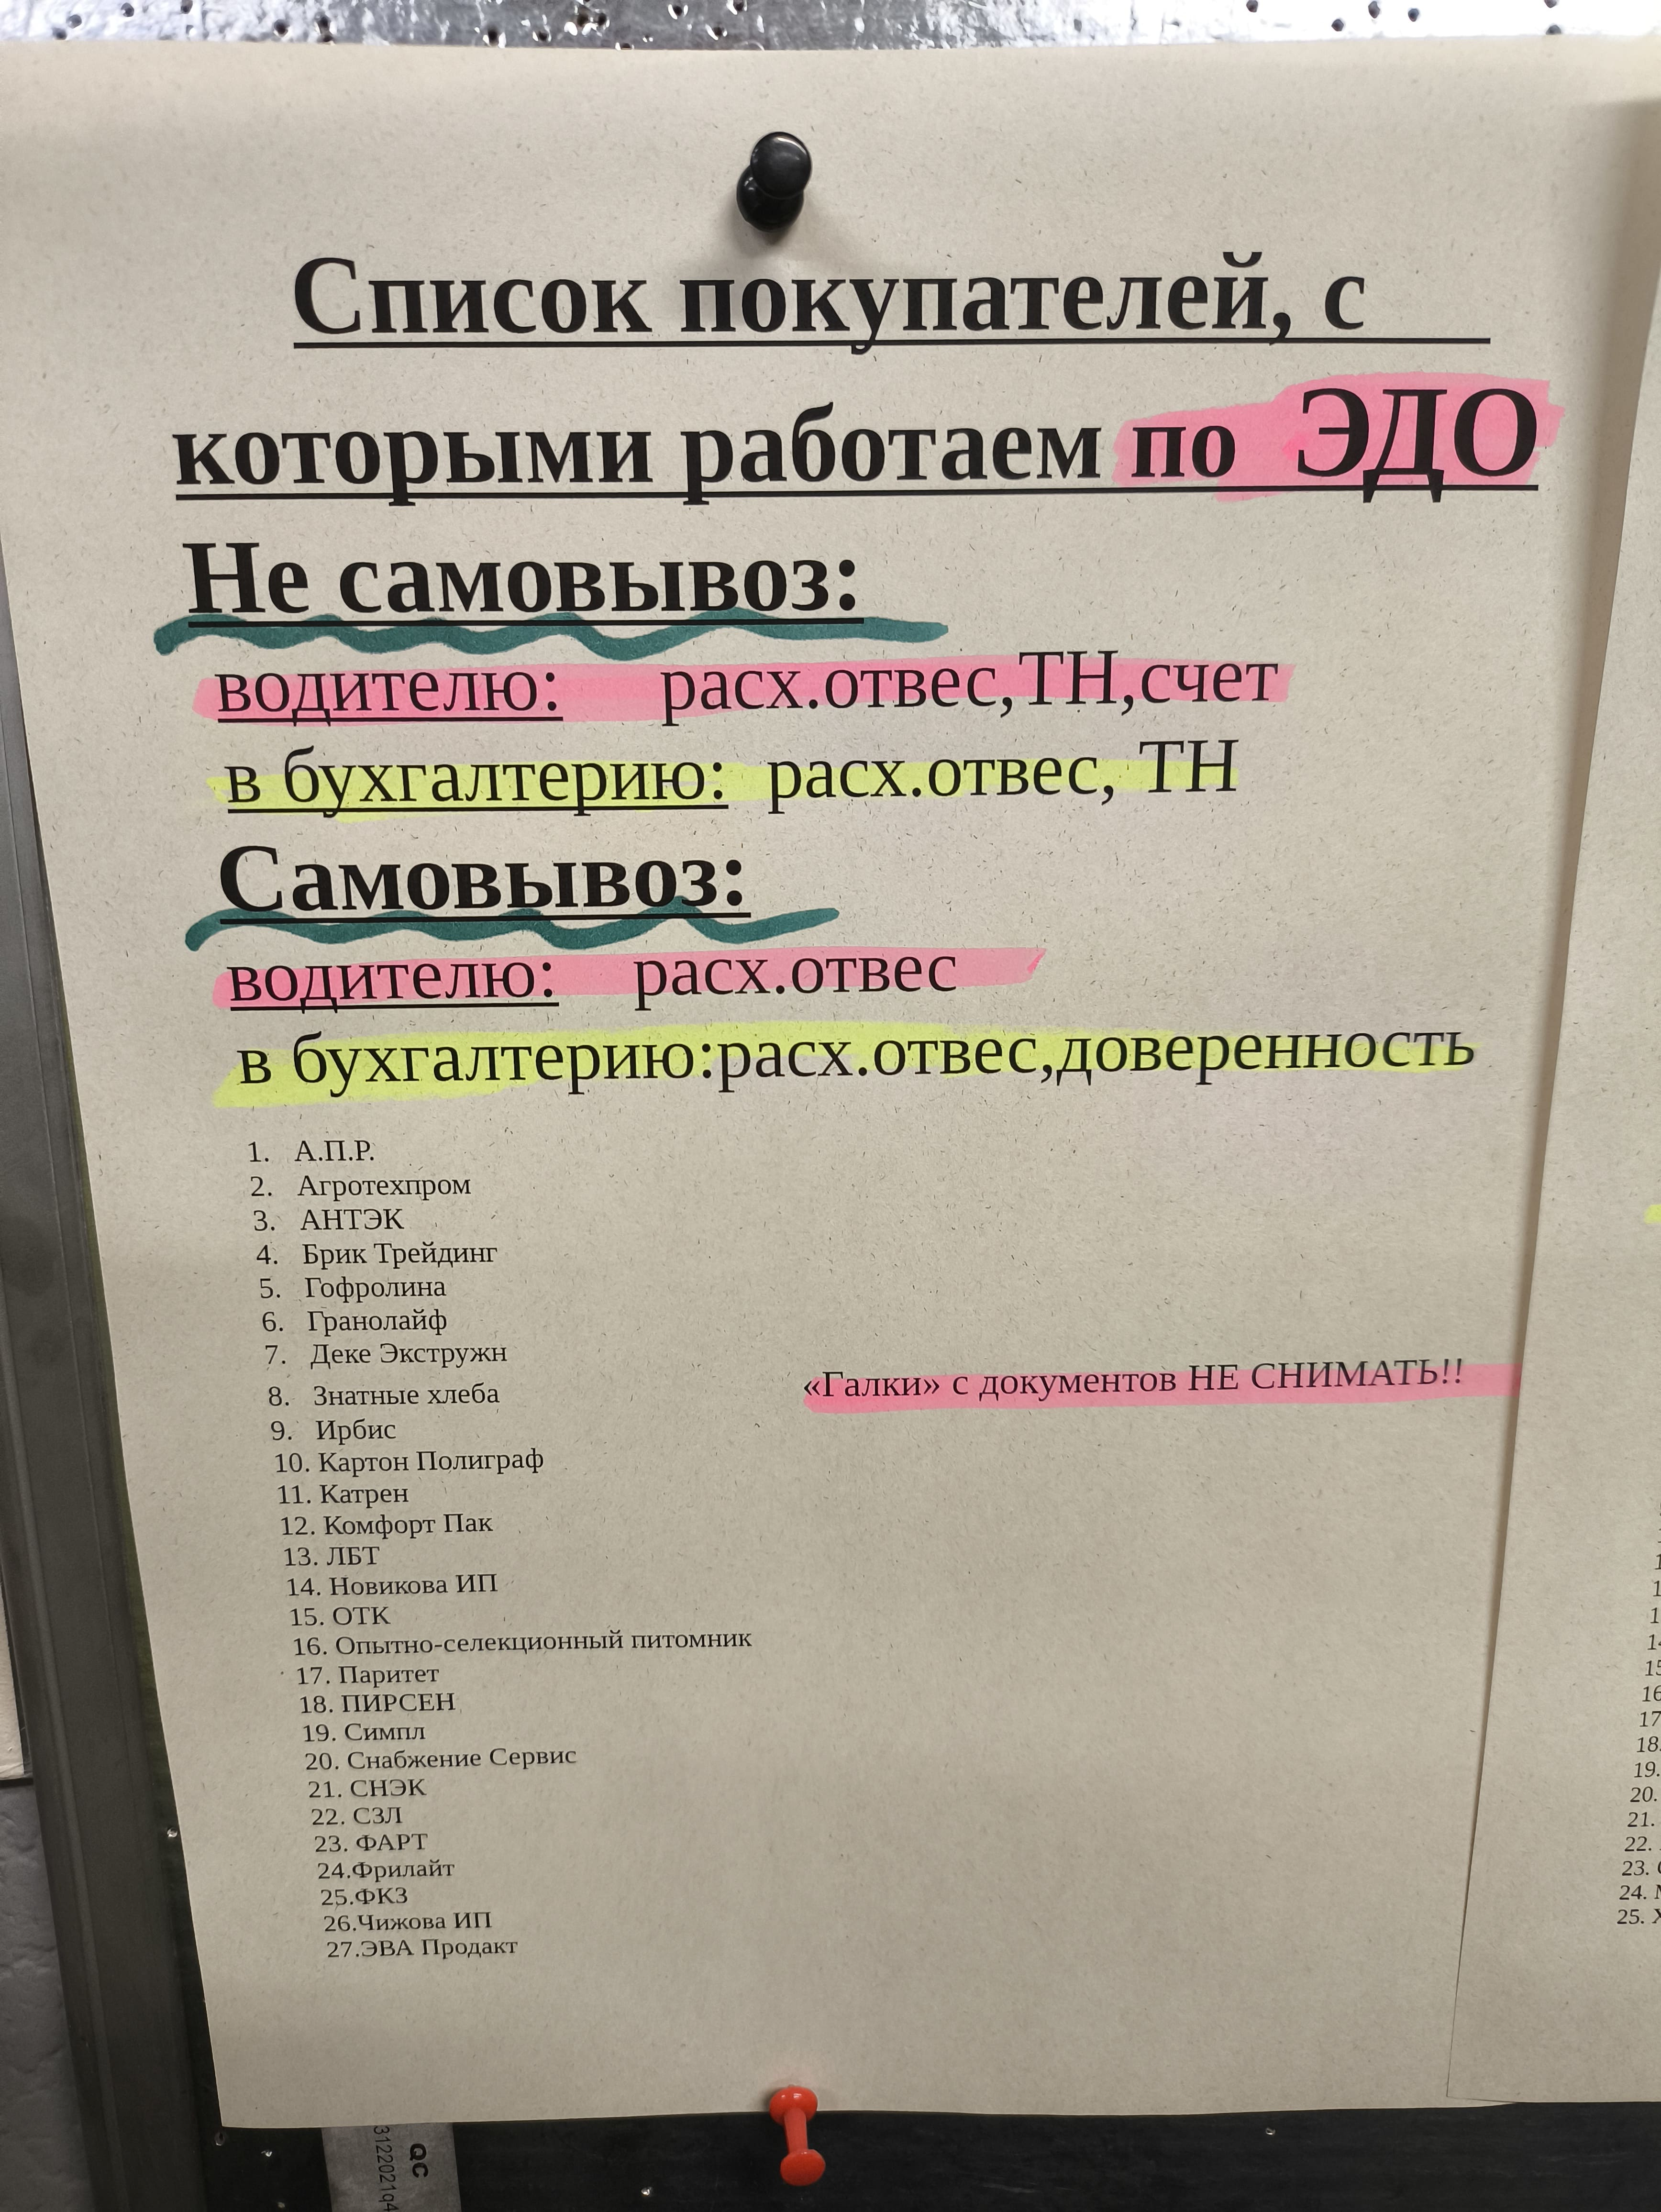
\includegraphics[height=0.6\textheight, keepaspectratio]{Pics/IX памятка кладовщикам.jpg}
\end{center}
 \caption{Памятка кладовщикам}
 \label{pic:IX памятка кладовщикам}
\end{figure}

\clearpage
% Графика подачи машин не выявлено. Машины на погрузку подъезжают в порядке очереди.
% По факту поступления машины кладовщик принимает машину. 
% Кладовщик грузит готовую продукцию по факту на основании плана погрузки и заявки из 1С. Остатки могут остаться на складе. 
% Кладовщик отмечает в заявке покупателя факт отгрузки, передает в отдел учета.

% Кладовщик по отгрузке или мастер смены ночью пишет накладную (рис. \ref{pic:d17}).
% Машина ночью грузится, но ее не отпускают.
% Кладовщик на площадке 1 пишет накладную (рис. \ref{pic:d18}), сканирует и высылает в отдел складской логистики. 
%  По второй площадке Кладовщики пишут заявку покупателя. 
% % (рис. \ref{pic:d19}).
% Кладовщик сам печатает другие бирки на складе по готовой продукции, меняет дату, клиента (рис. \ref{pic:d40}).

% В Google Tab Кладовщики меняет списание по факту.
% Существуют заявки от менеджеров, где указывается количество листов по готовой продукции (рис. \ref{pic:d41}).
% Менеджер может попросить отгрузить другое количество, чем указано в упаковке на паллете (рис. \ref{pic:d42}). Кладовщик может разукомплектовать чужой паллет при необходимости. При этом перепечатывает бирку.

 
% Кладовщик пишет накладную (рис. \ref{pic:d43}), сканирует, отправляет оператору по емайл. Оператор 1С создает в системе 1С: Бухгалтерия накладную, печатает сопроводительные документы, передает водителю.


% Отдел складской логистики на основании накладных (рис. \ref{pic:d17}, \ref{pic:d18})
% % или \ref{pic:d19}) 
% выписывает расходную накладную в системе 1С: Бухгалтерия (упр) и в реальной 1С: Бухгалтерия по юридическому лицу, указанному в заявке.
% В заявке на поставку указано юридическое лицо, от которого будет реализация.
% Отдел логистики печатает расходную накладную и при необходимости пакет сопроводительных документов.

% Паспорта качества по готовой продукции не печатаются.

% В течение дня 
% % по форме \ref{pic:d19}
% оператор 1С создает документ ''Отчет производства за смену''. На основании документа ''Реализация'' учетчик создает в системе 1С Бухгалтерия документ ''Перемещение'' с производства на склад и документ ''Реализация'' по факту отгрузки.

% По площадке 1 учетчик получает заявку на отгрузку. В системе 1С Бухгалтерия создает документ ''Поступление ТМЦ'', ''Перемещение'' и ''Реализация''. Форму накладной отсылает почтой на склад.
% Учетчик регистрирует поступление готовой продукции только в системе 1С Бухгалтерия (Упр). В информационной базе 1С по 
% ИМ Макаров учетчик создает только документ ''Реализация''. В информационной базе 1С по фирме  Норд-Пак учетчик создает документ ''Отчет производства за смену'' и документ ''Реализация''.




% \begin{figure}
% \begin{center}
%   \includegraphics[height=0.94\textheight, keepaspectratio]{Pics/d17.jpg}
% \end{center}
%   \caption{Накладная на отгрузку готовой продукции площадка 3}
%   \label{pic:d17}
% \end{figure}

% \begin{figure}
% \begin{center}
%   \includegraphics[height=0.94\textheight, keepaspectratio]{Pics/d18.jpg}
% \end{center}
%   \caption{Накладная на отгрузку готовой продукции площадка 1}
%   \label{pic:d18}
% \end{figure}




% \begin{figure}
% \begin{center}
%   \includegraphics[height=0.94\textheight, keepaspectratio]{Pics/d43.jpg}
% \end{center}
%   \caption{Накладная на отгрузку готовой продукции площадка 2}
%   \label{pic:d43}
% \end{figure}

%\clearpage